\section{Method}

\begin{figure*}[t]
    \centering
    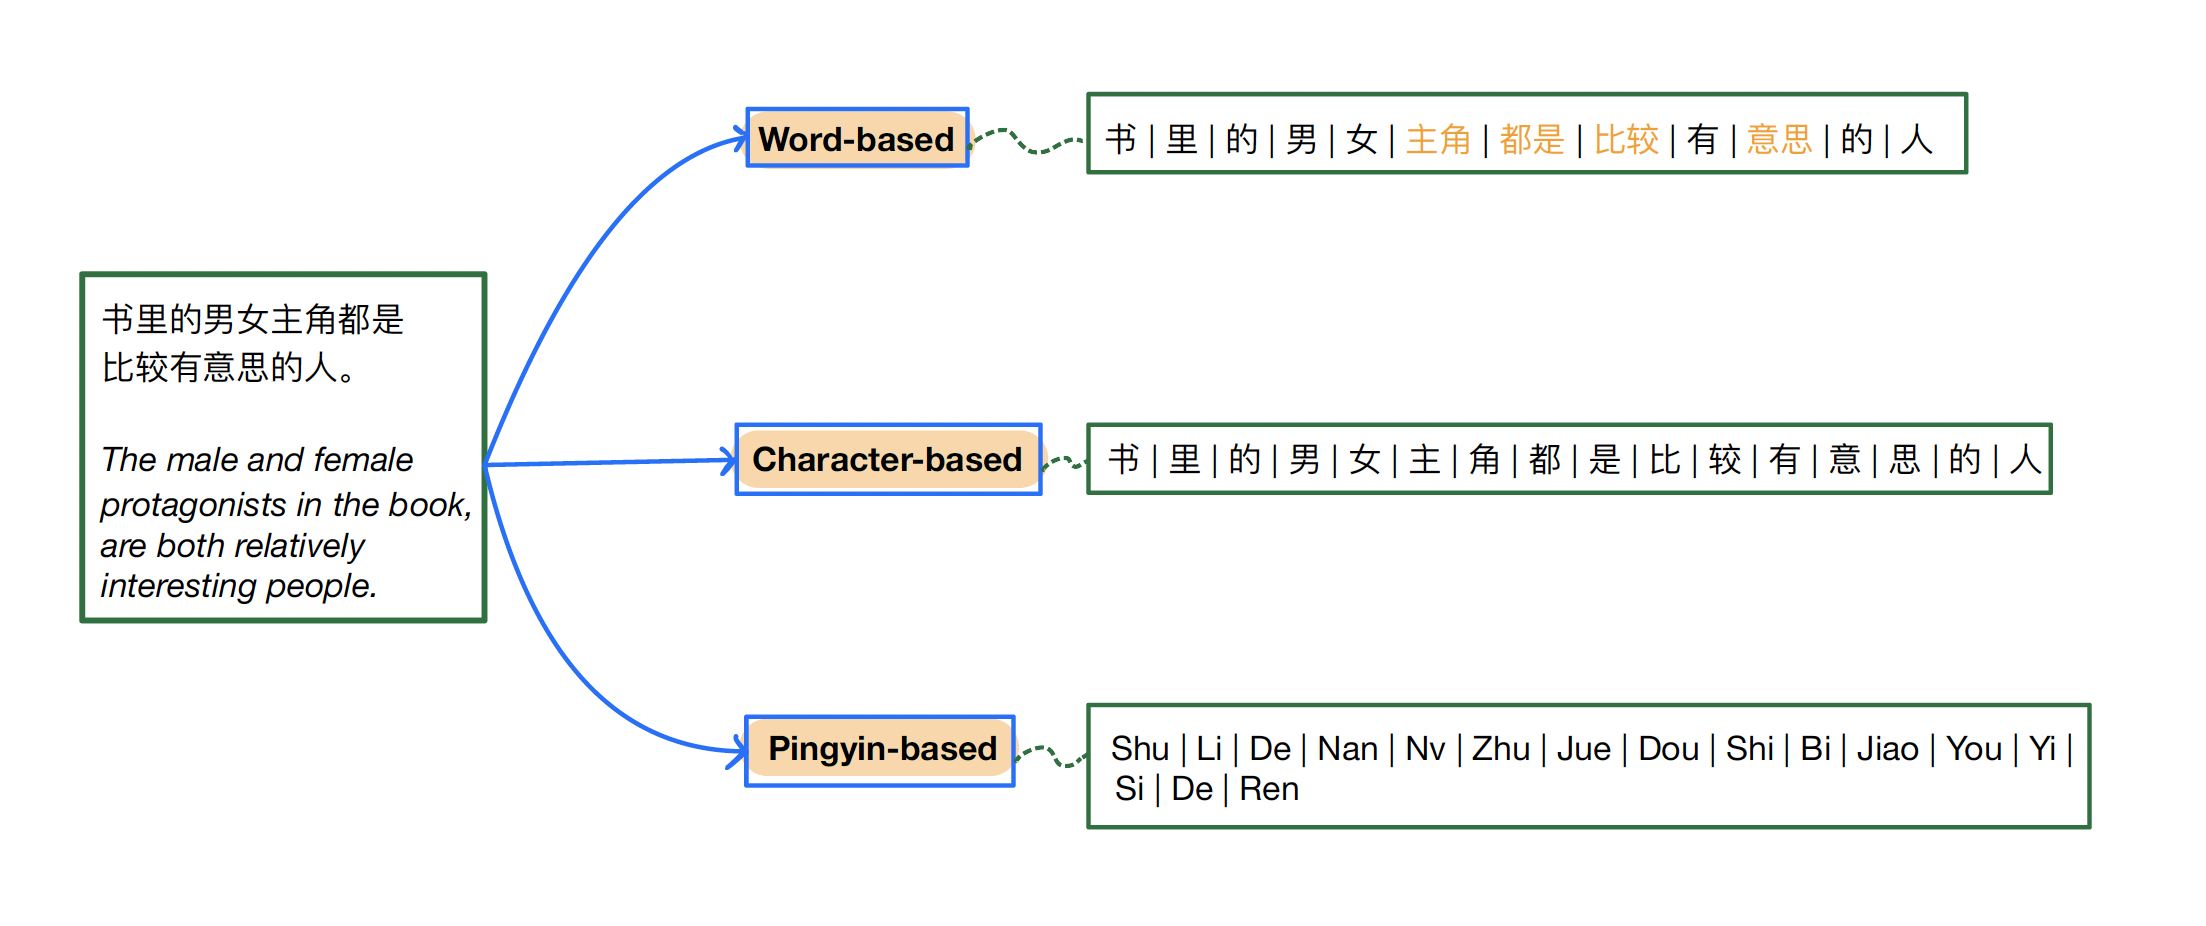
\includegraphics[width=14cm]{tokenization.png}
    \caption{Example of a sentence tokenized using different Chinese schemes: character level, word level, and pinyin level without tone.}
    \label{fig:figure1}
\end{figure*}

In this section, we describe the details of our implemented models, including LR, LSTM, BiLSTM, and a BiLSTM variant augmented with an attention layer. We also outline the dataset used for our experiments and provide details of applied data preprocessing methods.

\subsection{Logistic Regression}
The first model we implemented is LR, a statistical method designed for classification. This model predicts the likelihood of an input belonging to a certain category, using the logistic function for binary classification and the softmax function for multi-class scenarios. In our implementation, character-level tokenization was conducted straightforwardly, word-level tokenization was performed using \textit{Jieba}, and pinyin-level tokenization was carried out with the \textit{pinyin} package. The pinyin-level tokens employed do not contain tone information. For bigram feature extraction at the character level, we created bigrams directly from the character-level tokens. The features for the LR model is based on a bag-of-words approach, implemented using CountVectorizer from the \textit{sklearn} library. We trained the model with cross-entropy loss and implemented an early stopping mechanism that halts the training process if the validation loss doesn't improve for five successive epochs. The early stopping mechanism is crucial as it helps to avoid the model from overfitting to the training set. Additionally, we investigated the effect of removing Chinese stopwords, with results detailed in the Result section. 

\begin{table*}[ht]
\centering
\begin{tabular}{l l c c c c}
\hline
\textbf{Model} & \textbf{Tokenization} & \textbf{Stopword Removal} & \textbf{Vocab Size} & \textbf{Accuracy} & \textbf{F1 Score} \\ 
\hline
\hline
LR & Character & No & 4,694 & 90.30\% & 90.30\% \\
LR & Character-Bigram & No & 267,105 & \textbf{93.08\%} & \textbf{92.69\%} \\
LR & Word & No & 67,210 & 92.32\% & 92.34\% \\
LR & Pinyin & No & 501 & 85.19\% & 85.09\% \\
\hline
\hline
BiLSTM & \multirow{2}{*}{Character} & No & 4,884 & 91.85\% & 91.87\% \\
BiLSTM-w2v &  & No & 4,884 & 91.04\% & 91.20\% \\
\hline
BiLSTM & \multirow{2}{*}{Character-Bigram} & No & 304,936 & 90.57\% & 90.65\% \\
BiLSTM-w2v & & No & 304,936 & 90.42\% & 90.60\% \\
\hline
BiLSTM & \multirow{2}{*}{Word} & No & 68,495 & 90.80\% & 90.93\% \\
BiLSTM-w2v & & No & 68,495 & \textbf{92.02\%} & \textbf{91.73\%} \\
\hline
BiLSTM & Pinyin & No & 691 & 91.15\% & 91.18\% \\
\hline
\end{tabular}
\caption{Performance Comparison of LR and BiLSTM Models Using Four Tokenization Methods and Stopword Settings on \textit{onlineShopping10cats} Dataset for Sentiment Analysis}
\label{table:model_performance_sentiment}
\end{table*}


\subsection{LSTM and its variants}
We also implemented an LSTM model, tailored to address the challenges of long-range dependencies and contextual data interpretation, which is pivotal for text classification and sentiment analysis tasks~\citep{sun2022word, yuan2023}. LSTM processes text in sequence, dynamically updating its input, forget, and output states to preserve important previous context, a key factor in sentiment interpretation. Our LSTM integrates an embedding layer, potentially utilizing a pre-trained word2vec embedding, to convert tokens into vectors. The pretrained word2vec embedding\footnote{https://github.com/Embedding/Chinese-Word-Vectors/tree/master} we used, sourced from the study~\citep{li2018ana}, is capable of converting both words and characters into semantically meaningful vectors. This pretrained word2vec model covers 99.6\% of the characters in our dataset and approximately 70\% of the words resulting from \textit{Jieba}'s word-level tokenization. For the pinyin-level tokenization, word2vec embeddings is unavailable. In LSTM models that do not utilize the pretrained word2vec embedding, input tokens are initialized with random embeddings. The effectiveness of incorporating the word2vec embedding is examined in the Results section. Moreover, we evaluated the need for a bidirectional layer using the validation set. We refer to the bidirectional LSTM as BiLSTM, which is capable of capturing temporal dependencies in both forward and backward directions. The model finally utilizes a fully connected layer that assigns outputs from the LSTM layer into predefined categories. This design is effective in handling sequences of varying length.

Furthermore, we enhanced our BiLSTM model by incorporating an attention mechanism, referred to as BiLSTM\_A. The attention mechanism calculates attention scores using the outputs of hidden states from the LSTM layer, with a tanh activation and a linear projection. These scores are then used to weight the LSTM's outputs, creating a context vector that is then passed through the final layer to produce the ultimate classification results.

We employed the same tokenization schemes and bigram feature extraction methods for LSTM-based models same as we did for the LR model. In the training process, we applied the early stopping mechanism with a patience of five epochs and investigated the impact of stopwords removal for all LSTM models as well. Cross-entropy loss was utilized for training. We fine-tuned the hyper-parameters on the validation set, including the number of layers and the decision to use a bidirectional LSTM layer. Based on the model's performance with word-level tokenization, we selected two layers and a bidirectional structure. The embedding dimension was set to 300, in line with the pretrained word2vec embedding size. The final configuration for both BiLSTM and BiLSTM\_A models includes 128 hidden units, a dropout rate of 0.2, a learning rate of 0.003, and a batch size of 256.


\subsection{Dataset}
We conducted experiments on the \textit{onlineshopping10cats} dataset\footnote{https://github.com/SophonPlus/ChineseNlpCorpus/tree/master}, sourced from the ChineseNlpCorpus and uploaded in 2018. This dataset originates from user evaluations on an e-commerce website, and it contains 10 categories, including books, tablets, mobile phones, fruits, and more. This dataset comprises over 60,000 comments, equally balanced between positive and negative reviews and the 10 categories.

For data preprocessing, we first cleaned the data by removing punctuation marks and special symbols from the text. Optionally, we perform the removal of common Chinese stopwords, which are high-frequency words that do not contribute significantly to the meaning of the text. The stopwords are obtained from a GitHub repository\footnote{https://github.com/stopwords-iso/stopwords-zh}. For the purposes of model training and evaluation, the dataset was then divided: 70\% was used for training, 15\% for validation and model selection, and the remaining 15\% served as the test set. 


